\documentclass{article}
\usepackage{preamble}

\title{The $\sigma$-algebra inverse limit thing}
\author{Abhimanyu Pallavi Sudhir}
\date{13 November 2022}

\begin{document}

\maketitle

\section{Dummy}

\begin{definition}[Maximal Introspection -- single-observer]\label{def:introspection}

Let $\EVENT^0$ be a set, called the base partition, and define a sequence $\seq{\EVENT^n}$ by the following recurrence:

\begin{align*}
    \PROBS^{n} &= \set{\PROB : \EVENT^{n} \to [0, 1] \con \sum_{\event\in\EVENT^n}\PROB(\event)=1} \\
    \EVENT^{n+1} &= \EVENT^0 \times \PROBS^{n}
\end{align*}

($\PROBS^{n}$ should be read as the probability measure defined by ``the $(n+1)$-level agent on the $n$-level partition'') -- and define for $m\le n$ the projection $\proj^{mn}:\EVENT^n\to\EVENT^m$ transitively via composition on the following recurrence:

\begin{align*}
    \proj^{01}\bra{\event^0, \PROB^0} &= \event^0 \\
    \proj^{m(m+1)}\bra{\event^0, \PROB^m)} &= \tup{\event^0 \com 
    \function{\eventG}{\EVENT^{m-1}}{\sum_{\eventH\in\inv{\proj^{(m-1)m}}\left(\eventG\right)}{\PROB^m(\eventH)}}}
\end{align*}

Then $\seq{\EVENT^n}$ forms an inverse family under these connecting morphisms, and we call the inverse limit $\EVENT := \varprojlim \EVENT^n$ the ``maximally introspective extension'' of $\EVENT^0$.

\end{definition}

Concretely, an element of $\EVENT$ is an element of $\EVENT^0$ along with a sequence of probability distributions such that each successive probability distribution that ``refines'' the previous. Examples of ``interpreting''/coarsening an event in $\EVENT^{n+1}$ as an event in $\EVENT^n$ (because this is the tricky bit) in Figs~\ref{fig:proj01},~\ref{fig:proj12},~\ref{fig:proj23} respectively.

To be sure, this definition is pretty lacking -- it doesn't quite suffice for formulating G\"odel's theorem, because any program you place in $\EVENT^0$ is unable to refer to the agent's beliefs, which are located in the finer $\sigma$-algebras. A fuller description -- for an agent rather than an observer, and for multiple agents -- would require a more general (perhaps category-theoretic) definition, which would also provide a formal justification for this inverse-limit construction. I can probably do this fairly easily.

But this does provide us with a toy model to figure out exactly how an inverse-limit construction avoids Cantorian issues, whether this $\EVENT$ should be interpreted as a $\sigma$-algebra or a sample space, etc. 

\begin{figure}
    \centering
    \begin{tikzpicture}[x=0.75pt,y=0.75pt,yscale=-1,xscale=1]
%uncomment if require: \path (0,939); %set diagram left start at 0, and has height of 939

%Shape: Brace [id:dp251157528200062] 
\draw   (194,409.6) .. controls (197.84,409.6) and (199.76,407.68) .. (199.76,403.84) -- (199.76,403.84) .. controls (199.76,398.35) and (201.68,395.6) .. (205.53,395.6) .. controls (201.68,395.6) and (199.76,392.85) .. (199.76,387.36)(199.76,389.84) -- (199.76,387.36) .. controls (199.76,383.52) and (197.84,381.6) .. (194,381.6) ;
%Shape: Brace [id:dp7883937679306681] 
\draw   (194,452.6) .. controls (197.84,452.6) and (199.76,450.68) .. (199.76,446.84) -- (199.76,446.84) .. controls (199.76,441.35) and (201.68,438.6) .. (205.53,438.6) .. controls (201.68,438.6) and (199.76,435.85) .. (199.76,430.36)(199.76,432.84) -- (199.76,430.36) .. controls (199.76,426.52) and (197.84,424.6) .. (194,424.6) ;

% Text Node
\draw (179,386) node [anchor=north west][inner sep=0.75pt]    {$0$};
% Text Node
\draw (179,431) node [anchor=north west][inner sep=0.75pt]    {$1$};
% Text Node
\draw (220,386) node [anchor=north west][inner sep=0.75pt]  [color={rgb, 255:red, 200; green, 0; blue, 0 }  ,opacity=1 ]  {$0.5$};
% Text Node
\draw (219,431) node [anchor=north west][inner sep=0.75pt]  [color={rgb, 255:red, 200; green, 0; blue, 0 }  ,opacity=1 ]  {$0.5$};
% Text Node
\draw (355,409) node [anchor=north west][inner sep=0.75pt]    {$0$};
% Text Node
\draw (79,408) node [anchor=north west][inner sep=0.75pt]    {$\proj ^{01} \ \ :$};
% Text Node
\draw (295,408) node [anchor=north west][inner sep=0.75pt]    {$\mapsto $};
% Text Node
\draw (261,411) node [anchor=north west][inner sep=0.75pt]    {$0$};


\end{tikzpicture}

    \caption{$\proj^{01}$}
    \label{fig:proj01}
\end{figure}

\begin{figure}
    \centering
    \begin{tikzpicture}[x=0.75pt,y=0.75pt,yscale=-1,xscale=1]
%uncomment if require: \path (0,939); %set diagram left start at 0, and has height of 939

%Shape: Brace [id:dp8925717067579433] 
\draw   (194,226) .. controls (197.84,226) and (199.76,224.08) .. (199.76,220.24) -- (199.76,220.24) .. controls (199.76,214.75) and (201.68,212) .. (205.53,212) .. controls (201.68,212) and (199.76,209.25) .. (199.76,203.76)(199.76,206.24) -- (199.76,203.76) .. controls (199.76,199.92) and (197.84,198) .. (194,198) ;
%Shape: Brace [id:dp9930372575108133] 
\draw   (194,269) .. controls (197.84,269) and (199.76,267.08) .. (199.76,263.24) -- (199.76,263.24) .. controls (199.76,257.75) and (201.68,255) .. (205.53,255) .. controls (201.68,255) and (199.76,252.25) .. (199.76,246.76)(199.76,249.24) -- (199.76,246.76) .. controls (199.76,242.92) and (197.84,241) .. (194,241) ;
%Shape: Brace [id:dp49407212631862096] 
\draw   (272,267.6) .. controls (276.67,267.6) and (279,265.27) .. (279,260.6) -- (279,243.6) .. controls (279,236.93) and (281.33,233.6) .. (286,233.6) .. controls (281.33,233.6) and (279,230.27) .. (279,223.6)(279,226.6) -- (279,206.6) .. controls (279,201.93) and (276.67,199.6) .. (272,199.6) ;
%Shape: Brace [id:dp2642864901066977] 
\draw   (193,319) .. controls (196.84,319) and (198.76,317.08) .. (198.76,313.24) -- (198.76,313.24) .. controls (198.76,307.75) and (200.68,305) .. (204.53,305) .. controls (200.68,305) and (198.76,302.25) .. (198.76,296.76)(198.76,299.24) -- (198.76,296.76) .. controls (198.76,292.92) and (196.84,291) .. (193,291) ;
%Shape: Brace [id:dp19507790177064277] 
\draw   (193,362) .. controls (196.84,362) and (198.76,360.08) .. (198.76,356.24) -- (198.76,356.24) .. controls (198.76,350.75) and (200.68,348) .. (204.53,348) .. controls (200.68,348) and (198.76,345.25) .. (198.76,339.76)(198.76,342.24) -- (198.76,339.76) .. controls (198.76,335.92) and (196.84,334) .. (193,334) ;
%Shape: Brace [id:dp9825388835151163] 
\draw   (271,360.6) .. controls (275.67,360.6) and (278,358.27) .. (278,353.6) -- (278,336.6) .. controls (278,329.93) and (280.33,326.6) .. (285,326.6) .. controls (280.33,326.6) and (278,323.27) .. (278,316.6)(278,319.6) -- (278,299.6) .. controls (278,294.93) and (275.67,292.6) .. (271,292.6) ;
%Shape: Brace [id:dp6587423546374735] 
\draw   (192,405) .. controls (195.84,405) and (197.76,403.08) .. (197.76,399.24) -- (197.76,399.24) .. controls (197.76,393.75) and (199.68,391) .. (203.53,391) .. controls (199.68,391) and (197.76,388.25) .. (197.76,382.76)(197.76,385.24) -- (197.76,382.76) .. controls (197.76,378.92) and (195.84,377) .. (192,377) ;
%Shape: Brace [id:dp44253017121352056] 
\draw   (192,448) .. controls (195.84,448) and (197.76,446.08) .. (197.76,442.24) -- (197.76,442.24) .. controls (197.76,436.75) and (199.68,434) .. (203.53,434) .. controls (199.68,434) and (197.76,431.25) .. (197.76,425.76)(197.76,428.24) -- (197.76,425.76) .. controls (197.76,421.92) and (195.84,420) .. (192,420) ;
%Shape: Brace [id:dp07979164157526908] 
\draw   (270,446.6) .. controls (274.67,446.6) and (277,444.27) .. (277,439.6) -- (277,422.6) .. controls (277,415.93) and (279.33,412.6) .. (284,412.6) .. controls (279.33,412.6) and (277,409.27) .. (277,402.6)(277,405.6) -- (277,385.6) .. controls (277,380.93) and (274.67,378.6) .. (270,378.6) ;
%Shape: Brace [id:dp6553841544735148] 
\draw   (499,363) .. controls (502.84,363) and (504.76,361.08) .. (504.76,357.24) -- (504.76,357.24) .. controls (504.76,351.75) and (506.68,349) .. (510.53,349) .. controls (506.68,349) and (504.76,346.25) .. (504.76,340.76)(504.76,343.24) -- (504.76,340.76) .. controls (504.76,336.92) and (502.84,335) .. (499,335) ;
%Shape: Brace [id:dp5031123400583049] 
\draw   (499,406) .. controls (502.84,406) and (504.76,404.08) .. (504.76,400.24) -- (504.76,400.24) .. controls (504.76,394.75) and (506.68,392) .. (510.53,392) .. controls (506.68,392) and (504.76,389.25) .. (504.76,383.76)(504.76,386.24) -- (504.76,383.76) .. controls (504.76,379.92) and (502.84,378) .. (499,378) ;
%Shape: Brace [id:dp5448836891188555] 
\draw   (191,491) .. controls (194.84,491) and (196.76,489.08) .. (196.76,485.24) -- (196.76,485.24) .. controls (196.76,479.75) and (198.68,477) .. (202.53,477) .. controls (198.68,477) and (196.76,474.25) .. (196.76,468.76)(196.76,471.24) -- (196.76,468.76) .. controls (196.76,464.92) and (194.84,463) .. (191,463) ;
%Shape: Brace [id:dp1507272930476986] 
\draw   (191,534) .. controls (194.84,534) and (196.76,532.08) .. (196.76,528.24) -- (196.76,528.24) .. controls (196.76,522.75) and (198.68,520) .. (202.53,520) .. controls (198.68,520) and (196.76,517.25) .. (196.76,511.76)(196.76,514.24) -- (196.76,511.76) .. controls (196.76,507.92) and (194.84,506) .. (191,506) ;
%Shape: Brace [id:dp26665901097472156] 
\draw   (269,532.6) .. controls (273.67,532.6) and (276,530.27) .. (276,525.6) -- (276,508.6) .. controls (276,501.93) and (278.33,498.6) .. (283,498.6) .. controls (278.33,498.6) and (276,495.27) .. (276,488.6)(276,491.6) -- (276,471.6) .. controls (276,466.93) and (273.67,464.6) .. (269,464.6) ;

% Text Node
\draw (80,359.4) node [anchor=north west][inner sep=0.75pt]    {$\proj ^{12} \ \ :$};
% Text Node
\draw (179,202.4) node [anchor=north west][inner sep=0.75pt]    {$0$};
% Text Node
\draw (179,247.4) node [anchor=north west][inner sep=0.75pt]    {$1$};
% Text Node
\draw (220,202.4) node [anchor=north west][inner sep=0.75pt]  [color={rgb, 255:red, 200; green, 0; blue, 0 }  ,opacity=1 ]  {$0.5$};
% Text Node
\draw (219,247.4) node [anchor=north west][inner sep=0.75pt]  [color={rgb, 255:red, 200; green, 0; blue, 0 }  ,opacity=1 ]  {$0.5$};
% Text Node
\draw (260,224.4) node [anchor=north west][inner sep=0.75pt]    {$0$};
% Text Node
\draw (307,224.4) node [anchor=north west][inner sep=0.75pt]  [color={rgb, 255:red, 200; green, 0; blue, 0 }  ,opacity=1 ]  {$0.3$};
% Text Node
\draw (178,295.4) node [anchor=north west][inner sep=0.75pt]    {$0$};
% Text Node
\draw (178,340.4) node [anchor=north west][inner sep=0.75pt]    {$1$};
% Text Node
\draw (219,295.4) node [anchor=north west][inner sep=0.75pt]  [color={rgb, 255:red, 200; green, 0; blue, 0 }  ,opacity=1 ]  {$0.5$};
% Text Node
\draw (218,340.4) node [anchor=north west][inner sep=0.75pt]  [color={rgb, 255:red, 200; green, 0; blue, 0 }  ,opacity=1 ]  {$0.5$};
% Text Node
\draw (259,317.4) node [anchor=north west][inner sep=0.75pt]    {$1$};
% Text Node
\draw (306,317.4) node [anchor=north west][inner sep=0.75pt]  [color={rgb, 255:red, 200; green, 0; blue, 0 }  ,opacity=1 ]  {$0.4$};
% Text Node
\draw (177,381.4) node [anchor=north west][inner sep=0.75pt]    {$0$};
% Text Node
\draw (177,426.4) node [anchor=north west][inner sep=0.75pt]    {$1$};
% Text Node
\draw (218,381.4) node [anchor=north west][inner sep=0.75pt]  [color={rgb, 255:red, 200; green, 0; blue, 0 }  ,opacity=1 ]  {$0.1$};
% Text Node
\draw (217,426.4) node [anchor=north west][inner sep=0.75pt]  [color={rgb, 255:red, 200; green, 0; blue, 0 }  ,opacity=1 ]  {$0.9$};
% Text Node
\draw (258,403.4) node [anchor=north west][inner sep=0.75pt]    {$0$};
% Text Node
\draw (305,403.4) node [anchor=north west][inner sep=0.75pt]  [color={rgb, 255:red, 200; green, 0; blue, 0 }  ,opacity=1 ]  {$0.2$};
% Text Node
\draw (410,361.4) node [anchor=north west][inner sep=0.75pt]    {$\mapsto $};
% Text Node
\draw (484,339.4) node [anchor=north west][inner sep=0.75pt]    {$0$};
% Text Node
\draw (484,384.4) node [anchor=north west][inner sep=0.75pt]    {$1$};
% Text Node
\draw (525,339.4) node [anchor=north west][inner sep=0.75pt]  [color={rgb, 255:red, 200; green, 0; blue, 0 }  ,opacity=1 ]  {$0.5$};
% Text Node
\draw (524,384.4) node [anchor=north west][inner sep=0.75pt]  [color={rgb, 255:red, 200; green, 0; blue, 0 }  ,opacity=1 ]  {$0.5$};
% Text Node
\draw (176,467.4) node [anchor=north west][inner sep=0.75pt]    {$0$};
% Text Node
\draw (176,512.4) node [anchor=north west][inner sep=0.75pt]    {$1$};
% Text Node
\draw (217,467.4) node [anchor=north west][inner sep=0.75pt]  [color={rgb, 255:red, 200; green, 0; blue, 0 }  ,opacity=1 ]  {$0.1$};
% Text Node
\draw (216,512.4) node [anchor=north west][inner sep=0.75pt]  [color={rgb, 255:red, 200; green, 0; blue, 0 }  ,opacity=1 ]  {$0.9$};
% Text Node
\draw (257,489.4) node [anchor=north west][inner sep=0.75pt]    {$1$};
% Text Node
\draw (304,489.4) node [anchor=north west][inner sep=0.75pt]  [color={rgb, 255:red, 200; green, 0; blue, 0 }  ,opacity=1 ]  {$0.1$};
% Text Node
\draw (351,362.4) node [anchor=north west][inner sep=0.75pt]    {$0$};
% Text Node
\draw (575,357.4) node [anchor=north west][inner sep=0.75pt]    {$0$};


\end{tikzpicture}

    \caption{$\proj^{12}$}
    \label{fig:proj12}
\end{figure}

\begin{figure}
    \centering
    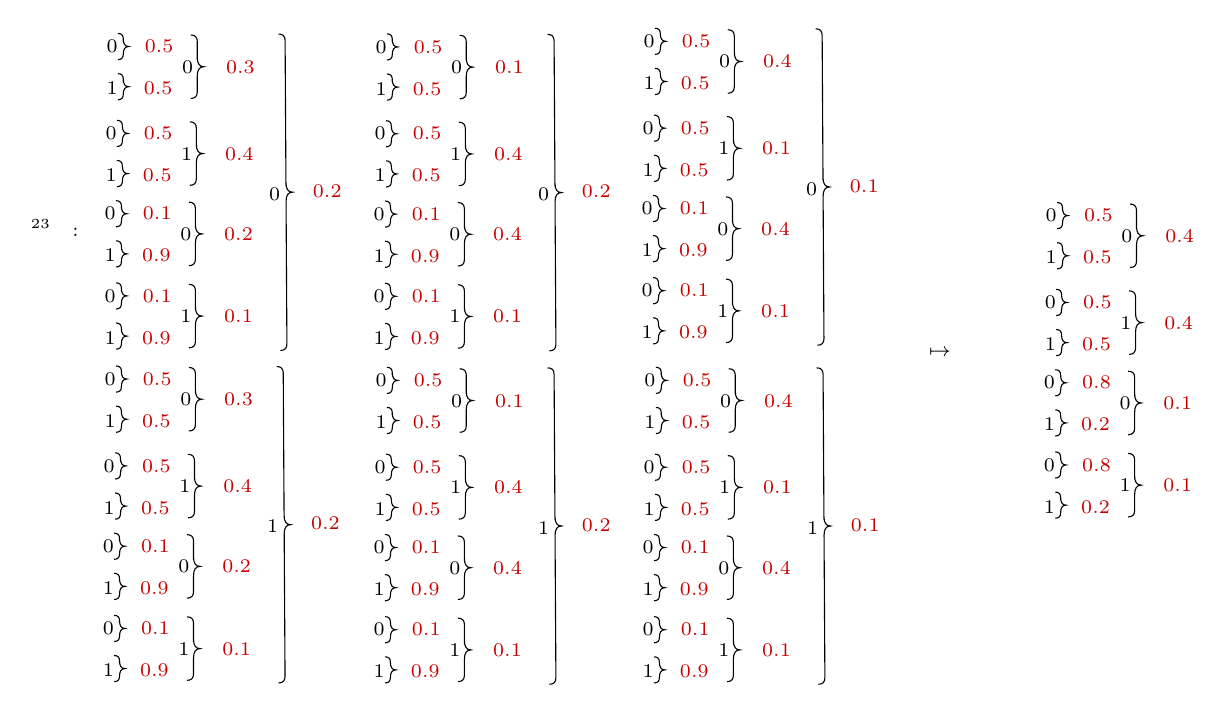
\begin{tikzpicture}[x=0.75pt,y=0.75pt,yscale=-0.45,xscale=0.45,font=\scriptsize]
%uncomment if require: \path (0,939); %set diagram left start at 0, and has height of 939

%Shape: Brace [id:dp58792179866058] 
\draw   (172,256.6) .. controls (175.84,256.6) and (177.76,254.68) .. (177.76,250.84) -- (177.76,250.84) .. controls (177.76,245.35) and (179.68,242.6) .. (183.53,242.6) .. controls (179.68,242.6) and (177.76,239.85) .. (177.76,234.36)(177.76,236.84) -- (177.76,234.36) .. controls (177.76,230.52) and (175.84,228.6) .. (172,228.6) ;
%Shape: Brace [id:dp4793644087069244] 
\draw   (172,299.6) .. controls (175.84,299.6) and (177.76,297.68) .. (177.76,293.84) -- (177.76,293.84) .. controls (177.76,288.35) and (179.68,285.6) .. (183.53,285.6) .. controls (179.68,285.6) and (177.76,282.85) .. (177.76,277.36)(177.76,279.84) -- (177.76,277.36) .. controls (177.76,273.52) and (175.84,271.6) .. (172,271.6) ;
%Shape: Brace [id:dp2745456297366389] 
\draw   (250,298.2) .. controls (254.67,298.2) and (257,295.87) .. (257,291.2) -- (257,274.2) .. controls (257,267.53) and (259.33,264.2) .. (264,264.2) .. controls (259.33,264.2) and (257,260.87) .. (257,254.2)(257,257.2) -- (257,237.2) .. controls (257,232.53) and (254.67,230.2) .. (250,230.2) ;
%Shape: Brace [id:dp8318546898868591] 
\draw   (171,349.6) .. controls (174.84,349.6) and (176.76,347.68) .. (176.76,343.84) -- (176.76,343.84) .. controls (176.76,338.35) and (178.68,335.6) .. (182.53,335.6) .. controls (178.68,335.6) and (176.76,332.85) .. (176.76,327.36)(176.76,329.84) -- (176.76,327.36) .. controls (176.76,323.52) and (174.84,321.6) .. (171,321.6) ;
%Shape: Brace [id:dp07865923951562248] 
\draw   (171,392.6) .. controls (174.84,392.6) and (176.76,390.68) .. (176.76,386.84) -- (176.76,386.84) .. controls (176.76,381.35) and (178.68,378.6) .. (182.53,378.6) .. controls (178.68,378.6) and (176.76,375.85) .. (176.76,370.36)(176.76,372.84) -- (176.76,370.36) .. controls (176.76,366.52) and (174.84,364.6) .. (171,364.6) ;
%Shape: Brace [id:dp7659753583174671] 
\draw   (249,391.2) .. controls (253.67,391.2) and (256,388.87) .. (256,384.2) -- (256,367.2) .. controls (256,360.53) and (258.33,357.2) .. (263,357.2) .. controls (258.33,357.2) and (256,353.87) .. (256,347.2)(256,350.2) -- (256,330.2) .. controls (256,325.53) and (253.67,323.2) .. (249,323.2) ;
%Shape: Brace [id:dp8970952283663483] 
\draw   (170,435.6) .. controls (173.84,435.6) and (175.76,433.68) .. (175.76,429.84) -- (175.76,429.84) .. controls (175.76,424.35) and (177.68,421.6) .. (181.53,421.6) .. controls (177.68,421.6) and (175.76,418.85) .. (175.76,413.36)(175.76,415.84) -- (175.76,413.36) .. controls (175.76,409.52) and (173.84,407.6) .. (170,407.6) ;
%Shape: Brace [id:dp557989321369958] 
\draw   (170,478.6) .. controls (173.84,478.6) and (175.76,476.68) .. (175.76,472.84) -- (175.76,472.84) .. controls (175.76,467.35) and (177.68,464.6) .. (181.53,464.6) .. controls (177.68,464.6) and (175.76,461.85) .. (175.76,456.36)(175.76,458.84) -- (175.76,456.36) .. controls (175.76,452.52) and (173.84,450.6) .. (170,450.6) ;
%Shape: Brace [id:dp5442944616784147] 
\draw   (248,477.2) .. controls (252.67,477.2) and (255,474.87) .. (255,470.2) -- (255,453.2) .. controls (255,446.53) and (257.33,443.2) .. (262,443.2) .. controls (257.33,443.2) and (255,439.87) .. (255,433.2)(255,436.2) -- (255,416.2) .. controls (255,411.53) and (252.67,409.2) .. (248,409.2) ;
%Shape: Brace [id:dp11172391152547534] 
\draw   (170,523.6) .. controls (173.84,523.6) and (175.76,521.68) .. (175.76,517.84) -- (175.76,517.84) .. controls (175.76,512.35) and (177.68,509.6) .. (181.53,509.6) .. controls (177.68,509.6) and (175.76,506.85) .. (175.76,501.36)(175.76,503.84) -- (175.76,501.36) .. controls (175.76,497.52) and (173.84,495.6) .. (170,495.6) ;
%Shape: Brace [id:dp3243436537585864] 
\draw   (170,566.6) .. controls (173.84,566.6) and (175.76,564.68) .. (175.76,560.84) -- (175.76,560.84) .. controls (175.76,555.35) and (177.68,552.6) .. (181.53,552.6) .. controls (177.68,552.6) and (175.76,549.85) .. (175.76,544.36)(175.76,546.84) -- (175.76,544.36) .. controls (175.76,540.52) and (173.84,538.6) .. (170,538.6) ;
%Shape: Brace [id:dp6179028534081237] 
\draw   (248,565.2) .. controls (252.67,565.2) and (255,562.87) .. (255,558.2) -- (255,541.2) .. controls (255,534.53) and (257.33,531.2) .. (262,531.2) .. controls (257.33,531.2) and (255,527.87) .. (255,521.2)(255,524.2) -- (255,504.2) .. controls (255,499.53) and (252.67,497.2) .. (248,497.2) ;
%Shape: Brace [id:dp445804565691275] 
\draw   (346,568) .. controls (350.67,567.97) and (352.99,565.63) .. (352.96,560.96) -- (352.05,408.56) .. controls (352.01,401.89) and (354.32,398.55) .. (358.99,398.52) .. controls (354.32,398.55) and (351.97,395.23) .. (351.94,388.56)(351.95,391.56) -- (351.03,236.16) .. controls (351,231.49) and (348.66,229.17) .. (343.99,229.2) ;
%Shape: Brace [id:dp7469301611280939] 
\draw   (170,612.6) .. controls (173.84,612.6) and (175.76,610.68) .. (175.76,606.84) -- (175.76,606.84) .. controls (175.76,601.35) and (177.68,598.6) .. (181.53,598.6) .. controls (177.68,598.6) and (175.76,595.85) .. (175.76,590.36)(175.76,592.84) -- (175.76,590.36) .. controls (175.76,586.52) and (173.84,584.6) .. (170,584.6) ;
%Shape: Brace [id:dp1560003659563638] 
\draw   (170,655.6) .. controls (173.84,655.6) and (175.76,653.68) .. (175.76,649.84) -- (175.76,649.84) .. controls (175.76,644.35) and (177.68,641.6) .. (181.53,641.6) .. controls (177.68,641.6) and (175.76,638.85) .. (175.76,633.36)(175.76,635.84) -- (175.76,633.36) .. controls (175.76,629.52) and (173.84,627.6) .. (170,627.6) ;
%Shape: Brace [id:dp5888841217822789] 
\draw   (248,654.2) .. controls (252.67,654.2) and (255,651.87) .. (255,647.2) -- (255,630.2) .. controls (255,623.53) and (257.33,620.2) .. (262,620.2) .. controls (257.33,620.2) and (255,616.87) .. (255,610.2)(255,613.2) -- (255,593.2) .. controls (255,588.53) and (252.67,586.2) .. (248,586.2) ;
%Shape: Brace [id:dp4871837858062582] 
\draw   (169,705.6) .. controls (172.84,705.6) and (174.76,703.68) .. (174.76,699.84) -- (174.76,699.84) .. controls (174.76,694.35) and (176.68,691.6) .. (180.53,691.6) .. controls (176.68,691.6) and (174.76,688.85) .. (174.76,683.36)(174.76,685.84) -- (174.76,683.36) .. controls (174.76,679.52) and (172.84,677.6) .. (169,677.6) ;
%Shape: Brace [id:dp895241148464242] 
\draw   (169,748.6) .. controls (172.84,748.6) and (174.76,746.68) .. (174.76,742.84) -- (174.76,742.84) .. controls (174.76,737.35) and (176.68,734.6) .. (180.53,734.6) .. controls (176.68,734.6) and (174.76,731.85) .. (174.76,726.36)(174.76,728.84) -- (174.76,726.36) .. controls (174.76,722.52) and (172.84,720.6) .. (169,720.6) ;
%Shape: Brace [id:dp6017053144160331] 
\draw   (247,747.2) .. controls (251.67,747.2) and (254,744.87) .. (254,740.2) -- (254,723.2) .. controls (254,716.53) and (256.33,713.2) .. (261,713.2) .. controls (256.33,713.2) and (254,709.87) .. (254,703.2)(254,706.2) -- (254,686.2) .. controls (254,681.53) and (251.67,679.2) .. (247,679.2) ;
%Shape: Brace [id:dp06432896075461825] 
\draw   (168,791.6) .. controls (171.84,791.6) and (173.76,789.68) .. (173.76,785.84) -- (173.76,785.84) .. controls (173.76,780.35) and (175.68,777.6) .. (179.53,777.6) .. controls (175.68,777.6) and (173.76,774.85) .. (173.76,769.36)(173.76,771.84) -- (173.76,769.36) .. controls (173.76,765.52) and (171.84,763.6) .. (168,763.6) ;
%Shape: Brace [id:dp920016930425839] 
\draw   (168,834.6) .. controls (171.84,834.6) and (173.76,832.68) .. (173.76,828.84) -- (173.76,828.84) .. controls (173.76,823.35) and (175.68,820.6) .. (179.53,820.6) .. controls (175.68,820.6) and (173.76,817.85) .. (173.76,812.36)(173.76,814.84) -- (173.76,812.36) .. controls (173.76,808.52) and (171.84,806.6) .. (168,806.6) ;
%Shape: Brace [id:dp4937313225031432] 
\draw   (246,833.2) .. controls (250.67,833.2) and (253,830.87) .. (253,826.2) -- (253,809.2) .. controls (253,802.53) and (255.33,799.2) .. (260,799.2) .. controls (255.33,799.2) and (253,795.87) .. (253,789.2)(253,792.2) -- (253,772.2) .. controls (253,767.53) and (250.67,765.2) .. (246,765.2) ;
%Shape: Brace [id:dp94308047208851] 
\draw   (168,879.6) .. controls (171.84,879.6) and (173.76,877.68) .. (173.76,873.84) -- (173.76,873.84) .. controls (173.76,868.35) and (175.68,865.6) .. (179.53,865.6) .. controls (175.68,865.6) and (173.76,862.85) .. (173.76,857.36)(173.76,859.84) -- (173.76,857.36) .. controls (173.76,853.52) and (171.84,851.6) .. (168,851.6) ;
%Shape: Brace [id:dp8890367060070803] 
\draw   (168,922.6) .. controls (171.84,922.6) and (173.76,920.68) .. (173.76,916.84) -- (173.76,916.84) .. controls (173.76,911.35) and (175.68,908.6) .. (179.53,908.6) .. controls (175.68,908.6) and (173.76,905.85) .. (173.76,900.36)(173.76,902.84) -- (173.76,900.36) .. controls (173.76,896.52) and (171.84,894.6) .. (168,894.6) ;
%Shape: Brace [id:dp18219271133141857] 
\draw   (246,921.2) .. controls (250.67,921.2) and (253,918.87) .. (253,914.2) -- (253,897.2) .. controls (253,890.53) and (255.33,887.2) .. (260,887.2) .. controls (255.33,887.2) and (253,883.87) .. (253,877.2)(253,880.2) -- (253,860.2) .. controls (253,855.53) and (250.67,853.2) .. (246,853.2) ;
%Shape: Brace [id:dp5430281489102862] 
\draw   (344,924) .. controls (348.67,923.97) and (350.99,921.63) .. (350.96,916.96) -- (350.05,764.56) .. controls (350.01,757.89) and (352.32,754.55) .. (356.99,754.52) .. controls (352.32,754.55) and (349.97,751.23) .. (349.94,744.56)(349.95,747.56) -- (349.03,592.16) .. controls (349,587.49) and (346.66,585.17) .. (341.99,585.2) ;
%Shape: Brace [id:dp6132329969465107] 
\draw   (460,257) .. controls (463.84,257) and (465.76,255.08) .. (465.76,251.24) -- (465.76,251.24) .. controls (465.76,245.75) and (467.68,243) .. (471.53,243) .. controls (467.68,243) and (465.76,240.25) .. (465.76,234.76)(465.76,237.24) -- (465.76,234.76) .. controls (465.76,230.92) and (463.84,229) .. (460,229) ;
%Shape: Brace [id:dp28574185019779175] 
\draw   (460,300) .. controls (463.84,300) and (465.76,298.08) .. (465.76,294.24) -- (465.76,294.24) .. controls (465.76,288.75) and (467.68,286) .. (471.53,286) .. controls (467.68,286) and (465.76,283.25) .. (465.76,277.76)(465.76,280.24) -- (465.76,277.76) .. controls (465.76,273.92) and (463.84,272) .. (460,272) ;
%Shape: Brace [id:dp20393823177363357] 
\draw   (538,298.6) .. controls (542.67,298.6) and (545,296.27) .. (545,291.6) -- (545,274.6) .. controls (545,267.93) and (547.33,264.6) .. (552,264.6) .. controls (547.33,264.6) and (545,261.27) .. (545,254.6)(545,257.6) -- (545,237.6) .. controls (545,232.93) and (542.67,230.6) .. (538,230.6) ;
%Shape: Brace [id:dp33203579861465227] 
\draw   (459,350) .. controls (462.84,350) and (464.76,348.08) .. (464.76,344.24) -- (464.76,344.24) .. controls (464.76,338.75) and (466.68,336) .. (470.53,336) .. controls (466.68,336) and (464.76,333.25) .. (464.76,327.76)(464.76,330.24) -- (464.76,327.76) .. controls (464.76,323.92) and (462.84,322) .. (459,322) ;
%Shape: Brace [id:dp5116953718447863] 
\draw   (459,393) .. controls (462.84,393) and (464.76,391.08) .. (464.76,387.24) -- (464.76,387.24) .. controls (464.76,381.75) and (466.68,379) .. (470.53,379) .. controls (466.68,379) and (464.76,376.25) .. (464.76,370.76)(464.76,373.24) -- (464.76,370.76) .. controls (464.76,366.92) and (462.84,365) .. (459,365) ;
%Shape: Brace [id:dp20253883495710667] 
\draw   (537,391.6) .. controls (541.67,391.6) and (544,389.27) .. (544,384.6) -- (544,367.6) .. controls (544,360.93) and (546.33,357.6) .. (551,357.6) .. controls (546.33,357.6) and (544,354.27) .. (544,347.6)(544,350.6) -- (544,330.6) .. controls (544,325.93) and (541.67,323.6) .. (537,323.6) ;
%Shape: Brace [id:dp0876603905768707] 
\draw   (458,436) .. controls (461.84,436) and (463.76,434.08) .. (463.76,430.24) -- (463.76,430.24) .. controls (463.76,424.75) and (465.68,422) .. (469.53,422) .. controls (465.68,422) and (463.76,419.25) .. (463.76,413.76)(463.76,416.24) -- (463.76,413.76) .. controls (463.76,409.92) and (461.84,408) .. (458,408) ;
%Shape: Brace [id:dp30071168081871136] 
\draw   (458,479) .. controls (461.84,479) and (463.76,477.08) .. (463.76,473.24) -- (463.76,473.24) .. controls (463.76,467.75) and (465.68,465) .. (469.53,465) .. controls (465.68,465) and (463.76,462.25) .. (463.76,456.76)(463.76,459.24) -- (463.76,456.76) .. controls (463.76,452.92) and (461.84,451) .. (458,451) ;
%Shape: Brace [id:dp7599471323197944] 
\draw   (536,477.6) .. controls (540.67,477.6) and (543,475.27) .. (543,470.6) -- (543,453.6) .. controls (543,446.93) and (545.33,443.6) .. (550,443.6) .. controls (545.33,443.6) and (543,440.27) .. (543,433.6)(543,436.6) -- (543,416.6) .. controls (543,411.93) and (540.67,409.6) .. (536,409.6) ;
%Shape: Brace [id:dp3531091008727092] 
\draw   (458,524) .. controls (461.84,524) and (463.76,522.08) .. (463.76,518.24) -- (463.76,518.24) .. controls (463.76,512.75) and (465.68,510) .. (469.53,510) .. controls (465.68,510) and (463.76,507.25) .. (463.76,501.76)(463.76,504.24) -- (463.76,501.76) .. controls (463.76,497.92) and (461.84,496) .. (458,496) ;
%Shape: Brace [id:dp36950680613413445] 
\draw   (458,567) .. controls (461.84,567) and (463.76,565.08) .. (463.76,561.24) -- (463.76,561.24) .. controls (463.76,555.75) and (465.68,553) .. (469.53,553) .. controls (465.68,553) and (463.76,550.25) .. (463.76,544.76)(463.76,547.24) -- (463.76,544.76) .. controls (463.76,540.92) and (461.84,539) .. (458,539) ;
%Shape: Brace [id:dp6961593907915491] 
\draw   (536,565.6) .. controls (540.67,565.6) and (543,563.27) .. (543,558.6) -- (543,541.6) .. controls (543,534.93) and (545.33,531.6) .. (550,531.6) .. controls (545.33,531.6) and (543,528.27) .. (543,521.6)(543,524.6) -- (543,504.6) .. controls (543,499.93) and (540.67,497.6) .. (536,497.6) ;
%Shape: Brace [id:dp3469988947997682] 
\draw   (634,568.4) .. controls (638.67,568.37) and (640.99,566.03) .. (640.96,561.36) -- (640.05,408.96) .. controls (640.01,402.29) and (642.32,398.95) .. (646.99,398.92) .. controls (642.32,398.95) and (639.97,395.63) .. (639.94,388.96)(639.95,391.96) -- (639.03,236.56) .. controls (639,231.89) and (636.66,229.57) .. (631.99,229.6) ;
%Shape: Brace [id:dp48998052978324824] 
\draw   (460,614) .. controls (463.84,614) and (465.76,612.08) .. (465.76,608.24) -- (465.76,608.24) .. controls (465.76,602.75) and (467.68,600) .. (471.53,600) .. controls (467.68,600) and (465.76,597.25) .. (465.76,591.76)(465.76,594.24) -- (465.76,591.76) .. controls (465.76,587.92) and (463.84,586) .. (460,586) ;
%Shape: Brace [id:dp746186209256249] 
\draw   (460,657) .. controls (463.84,657) and (465.76,655.08) .. (465.76,651.24) -- (465.76,651.24) .. controls (465.76,645.75) and (467.68,643) .. (471.53,643) .. controls (467.68,643) and (465.76,640.25) .. (465.76,634.76)(465.76,637.24) -- (465.76,634.76) .. controls (465.76,630.92) and (463.84,629) .. (460,629) ;
%Shape: Brace [id:dp886186257332449] 
\draw   (538,655.6) .. controls (542.67,655.6) and (545,653.27) .. (545,648.6) -- (545,631.6) .. controls (545,624.93) and (547.33,621.6) .. (552,621.6) .. controls (547.33,621.6) and (545,618.27) .. (545,611.6)(545,614.6) -- (545,594.6) .. controls (545,589.93) and (542.67,587.6) .. (538,587.6) ;
%Shape: Brace [id:dp4620849096973667] 
\draw   (459,707) .. controls (462.84,707) and (464.76,705.08) .. (464.76,701.24) -- (464.76,701.24) .. controls (464.76,695.75) and (466.68,693) .. (470.53,693) .. controls (466.68,693) and (464.76,690.25) .. (464.76,684.76)(464.76,687.24) -- (464.76,684.76) .. controls (464.76,680.92) and (462.84,679) .. (459,679) ;
%Shape: Brace [id:dp8427918270887655] 
\draw   (459,750) .. controls (462.84,750) and (464.76,748.08) .. (464.76,744.24) -- (464.76,744.24) .. controls (464.76,738.75) and (466.68,736) .. (470.53,736) .. controls (466.68,736) and (464.76,733.25) .. (464.76,727.76)(464.76,730.24) -- (464.76,727.76) .. controls (464.76,723.92) and (462.84,722) .. (459,722) ;
%Shape: Brace [id:dp2962708372255203] 
\draw   (537,748.6) .. controls (541.67,748.6) and (544,746.27) .. (544,741.6) -- (544,724.6) .. controls (544,717.93) and (546.33,714.6) .. (551,714.6) .. controls (546.33,714.6) and (544,711.27) .. (544,704.6)(544,707.6) -- (544,687.6) .. controls (544,682.93) and (541.67,680.6) .. (537,680.6) ;
%Shape: Brace [id:dp31637797360457975] 
\draw   (458,793) .. controls (461.84,793) and (463.76,791.08) .. (463.76,787.24) -- (463.76,787.24) .. controls (463.76,781.75) and (465.68,779) .. (469.53,779) .. controls (465.68,779) and (463.76,776.25) .. (463.76,770.76)(463.76,773.24) -- (463.76,770.76) .. controls (463.76,766.92) and (461.84,765) .. (458,765) ;
%Shape: Brace [id:dp47623734306579757] 
\draw   (458,836) .. controls (461.84,836) and (463.76,834.08) .. (463.76,830.24) -- (463.76,830.24) .. controls (463.76,824.75) and (465.68,822) .. (469.53,822) .. controls (465.68,822) and (463.76,819.25) .. (463.76,813.76)(463.76,816.24) -- (463.76,813.76) .. controls (463.76,809.92) and (461.84,808) .. (458,808) ;
%Shape: Brace [id:dp1324597638966043] 
\draw   (536,834.6) .. controls (540.67,834.6) and (543,832.27) .. (543,827.6) -- (543,810.6) .. controls (543,803.93) and (545.33,800.6) .. (550,800.6) .. controls (545.33,800.6) and (543,797.27) .. (543,790.6)(543,793.6) -- (543,773.6) .. controls (543,768.93) and (540.67,766.6) .. (536,766.6) ;
%Shape: Brace [id:dp8446851373868742] 
\draw   (458,881) .. controls (461.84,881) and (463.76,879.08) .. (463.76,875.24) -- (463.76,875.24) .. controls (463.76,869.75) and (465.68,867) .. (469.53,867) .. controls (465.68,867) and (463.76,864.25) .. (463.76,858.76)(463.76,861.24) -- (463.76,858.76) .. controls (463.76,854.92) and (461.84,853) .. (458,853) ;
%Shape: Brace [id:dp12999115538478967] 
\draw   (458,924) .. controls (461.84,924) and (463.76,922.08) .. (463.76,918.24) -- (463.76,918.24) .. controls (463.76,912.75) and (465.68,910) .. (469.53,910) .. controls (465.68,910) and (463.76,907.25) .. (463.76,901.76)(463.76,904.24) -- (463.76,901.76) .. controls (463.76,897.92) and (461.84,896) .. (458,896) ;
%Shape: Brace [id:dp2009043442455689] 
\draw   (536,922.6) .. controls (540.67,922.6) and (543,920.27) .. (543,915.6) -- (543,898.6) .. controls (543,891.93) and (545.33,888.6) .. (550,888.6) .. controls (545.33,888.6) and (543,885.27) .. (543,878.6)(543,881.6) -- (543,861.6) .. controls (543,856.93) and (540.67,854.6) .. (536,854.6) ;
%Shape: Brace [id:dp6846611189768357] 
\draw   (634,925.4) .. controls (638.67,925.37) and (640.99,923.03) .. (640.96,918.36) -- (640.05,765.96) .. controls (640.01,759.29) and (642.32,755.95) .. (646.99,755.92) .. controls (642.32,755.95) and (639.97,752.63) .. (639.94,745.96)(639.95,748.96) -- (639.03,593.56) .. controls (639,588.89) and (636.66,586.57) .. (631.99,586.6) ;
%Shape: Brace [id:dp1897210687061881] 
\draw   (747,251) .. controls (750.84,251) and (752.76,249.08) .. (752.76,245.24) -- (752.76,245.24) .. controls (752.76,239.75) and (754.68,237) .. (758.53,237) .. controls (754.68,237) and (752.76,234.25) .. (752.76,228.76)(752.76,231.24) -- (752.76,228.76) .. controls (752.76,224.92) and (750.84,223) .. (747,223) ;
%Shape: Brace [id:dp8653813909578592] 
\draw   (747,294) .. controls (750.84,294) and (752.76,292.08) .. (752.76,288.24) -- (752.76,288.24) .. controls (752.76,282.75) and (754.68,280) .. (758.53,280) .. controls (754.68,280) and (752.76,277.25) .. (752.76,271.76)(752.76,274.24) -- (752.76,271.76) .. controls (752.76,267.92) and (750.84,266) .. (747,266) ;
%Shape: Brace [id:dp7590428810962722] 
\draw   (825,292.6) .. controls (829.67,292.6) and (832,290.27) .. (832,285.6) -- (832,268.6) .. controls (832,261.93) and (834.33,258.6) .. (839,258.6) .. controls (834.33,258.6) and (832,255.27) .. (832,248.6)(832,251.6) -- (832,231.6) .. controls (832,226.93) and (829.67,224.6) .. (825,224.6) ;
%Shape: Brace [id:dp260234041735641] 
\draw   (746,344) .. controls (749.84,344) and (751.76,342.08) .. (751.76,338.24) -- (751.76,338.24) .. controls (751.76,332.75) and (753.68,330) .. (757.53,330) .. controls (753.68,330) and (751.76,327.25) .. (751.76,321.76)(751.76,324.24) -- (751.76,321.76) .. controls (751.76,317.92) and (749.84,316) .. (746,316) ;
%Shape: Brace [id:dp8234924460379474] 
\draw   (746,387) .. controls (749.84,387) and (751.76,385.08) .. (751.76,381.24) -- (751.76,381.24) .. controls (751.76,375.75) and (753.68,373) .. (757.53,373) .. controls (753.68,373) and (751.76,370.25) .. (751.76,364.76)(751.76,367.24) -- (751.76,364.76) .. controls (751.76,360.92) and (749.84,359) .. (746,359) ;
%Shape: Brace [id:dp5625815392918698] 
\draw   (824,385.6) .. controls (828.67,385.6) and (831,383.27) .. (831,378.6) -- (831,361.6) .. controls (831,354.93) and (833.33,351.6) .. (838,351.6) .. controls (833.33,351.6) and (831,348.27) .. (831,341.6)(831,344.6) -- (831,324.6) .. controls (831,319.93) and (828.67,317.6) .. (824,317.6) ;
%Shape: Brace [id:dp4311521260731559] 
\draw   (745,430) .. controls (748.84,430) and (750.76,428.08) .. (750.76,424.24) -- (750.76,424.24) .. controls (750.76,418.75) and (752.68,416) .. (756.53,416) .. controls (752.68,416) and (750.76,413.25) .. (750.76,407.76)(750.76,410.24) -- (750.76,407.76) .. controls (750.76,403.92) and (748.84,402) .. (745,402) ;
%Shape: Brace [id:dp7343802761070315] 
\draw   (745,473) .. controls (748.84,473) and (750.76,471.08) .. (750.76,467.24) -- (750.76,467.24) .. controls (750.76,461.75) and (752.68,459) .. (756.53,459) .. controls (752.68,459) and (750.76,456.25) .. (750.76,450.76)(750.76,453.24) -- (750.76,450.76) .. controls (750.76,446.92) and (748.84,445) .. (745,445) ;
%Shape: Brace [id:dp18771849680635522] 
\draw   (823,471.6) .. controls (827.67,471.6) and (830,469.27) .. (830,464.6) -- (830,447.6) .. controls (830,440.93) and (832.33,437.6) .. (837,437.6) .. controls (832.33,437.6) and (830,434.27) .. (830,427.6)(830,430.6) -- (830,410.6) .. controls (830,405.93) and (827.67,403.6) .. (823,403.6) ;
%Shape: Brace [id:dp6661458194844769] 
\draw   (745,518) .. controls (748.84,518) and (750.76,516.08) .. (750.76,512.24) -- (750.76,512.24) .. controls (750.76,506.75) and (752.68,504) .. (756.53,504) .. controls (752.68,504) and (750.76,501.25) .. (750.76,495.76)(750.76,498.24) -- (750.76,495.76) .. controls (750.76,491.92) and (748.84,490) .. (745,490) ;
%Shape: Brace [id:dp9112076106292903] 
\draw   (745,561) .. controls (748.84,561) and (750.76,559.08) .. (750.76,555.24) -- (750.76,555.24) .. controls (750.76,549.75) and (752.68,547) .. (756.53,547) .. controls (752.68,547) and (750.76,544.25) .. (750.76,538.76)(750.76,541.24) -- (750.76,538.76) .. controls (750.76,534.92) and (748.84,533) .. (745,533) ;
%Shape: Brace [id:dp7882115291512575] 
\draw   (823,559.6) .. controls (827.67,559.6) and (830,557.27) .. (830,552.6) -- (830,535.6) .. controls (830,528.93) and (832.33,525.6) .. (837,525.6) .. controls (832.33,525.6) and (830,522.27) .. (830,515.6)(830,518.6) -- (830,498.6) .. controls (830,493.93) and (827.67,491.6) .. (823,491.6) ;
%Shape: Brace [id:dp576212727956551] 
\draw   (921,562.4) .. controls (925.67,562.37) and (927.99,560.03) .. (927.96,555.36) -- (927.05,402.96) .. controls (927.01,396.29) and (929.32,392.95) .. (933.99,392.92) .. controls (929.32,392.95) and (926.97,389.63) .. (926.94,382.96)(926.95,385.96) -- (926.03,230.56) .. controls (926,225.89) and (923.66,223.57) .. (918.99,223.6) ;
%Shape: Brace [id:dp005388659970078535] 
\draw   (748,614) .. controls (751.84,614) and (753.76,612.08) .. (753.76,608.24) -- (753.76,608.24) .. controls (753.76,602.75) and (755.68,600) .. (759.53,600) .. controls (755.68,600) and (753.76,597.25) .. (753.76,591.76)(753.76,594.24) -- (753.76,591.76) .. controls (753.76,587.92) and (751.84,586) .. (748,586) ;
%Shape: Brace [id:dp01999969407451041] 
\draw   (748,657) .. controls (751.84,657) and (753.76,655.08) .. (753.76,651.24) -- (753.76,651.24) .. controls (753.76,645.75) and (755.68,643) .. (759.53,643) .. controls (755.68,643) and (753.76,640.25) .. (753.76,634.76)(753.76,637.24) -- (753.76,634.76) .. controls (753.76,630.92) and (751.84,629) .. (748,629) ;
%Shape: Brace [id:dp14402796357276682] 
\draw   (826,655.6) .. controls (830.67,655.6) and (833,653.27) .. (833,648.6) -- (833,631.6) .. controls (833,624.93) and (835.33,621.6) .. (840,621.6) .. controls (835.33,621.6) and (833,618.27) .. (833,611.6)(833,614.6) -- (833,594.6) .. controls (833,589.93) and (830.67,587.6) .. (826,587.6) ;
%Shape: Brace [id:dp47544507331510877] 
\draw   (747,707) .. controls (750.84,707) and (752.76,705.08) .. (752.76,701.24) -- (752.76,701.24) .. controls (752.76,695.75) and (754.68,693) .. (758.53,693) .. controls (754.68,693) and (752.76,690.25) .. (752.76,684.76)(752.76,687.24) -- (752.76,684.76) .. controls (752.76,680.92) and (750.84,679) .. (747,679) ;
%Shape: Brace [id:dp20988183134476324] 
\draw   (747,750) .. controls (750.84,750) and (752.76,748.08) .. (752.76,744.24) -- (752.76,744.24) .. controls (752.76,738.75) and (754.68,736) .. (758.53,736) .. controls (754.68,736) and (752.76,733.25) .. (752.76,727.76)(752.76,730.24) -- (752.76,727.76) .. controls (752.76,723.92) and (750.84,722) .. (747,722) ;
%Shape: Brace [id:dp9277295626008961] 
\draw   (825,748.6) .. controls (829.67,748.6) and (832,746.27) .. (832,741.6) -- (832,724.6) .. controls (832,717.93) and (834.33,714.6) .. (839,714.6) .. controls (834.33,714.6) and (832,711.27) .. (832,704.6)(832,707.6) -- (832,687.6) .. controls (832,682.93) and (829.67,680.6) .. (825,680.6) ;
%Shape: Brace [id:dp29071755086150763] 
\draw   (746,793) .. controls (749.84,793) and (751.76,791.08) .. (751.76,787.24) -- (751.76,787.24) .. controls (751.76,781.75) and (753.68,779) .. (757.53,779) .. controls (753.68,779) and (751.76,776.25) .. (751.76,770.76)(751.76,773.24) -- (751.76,770.76) .. controls (751.76,766.92) and (749.84,765) .. (746,765) ;
%Shape: Brace [id:dp33544563632364155] 
\draw   (746,836) .. controls (749.84,836) and (751.76,834.08) .. (751.76,830.24) -- (751.76,830.24) .. controls (751.76,824.75) and (753.68,822) .. (757.53,822) .. controls (753.68,822) and (751.76,819.25) .. (751.76,813.76)(751.76,816.24) -- (751.76,813.76) .. controls (751.76,809.92) and (749.84,808) .. (746,808) ;
%Shape: Brace [id:dp3145282637403253] 
\draw   (824,834.6) .. controls (828.67,834.6) and (831,832.27) .. (831,827.6) -- (831,810.6) .. controls (831,803.93) and (833.33,800.6) .. (838,800.6) .. controls (833.33,800.6) and (831,797.27) .. (831,790.6)(831,793.6) -- (831,773.6) .. controls (831,768.93) and (828.67,766.6) .. (824,766.6) ;
%Shape: Brace [id:dp6254748875584435] 
\draw   (746,881) .. controls (749.84,881) and (751.76,879.08) .. (751.76,875.24) -- (751.76,875.24) .. controls (751.76,869.75) and (753.68,867) .. (757.53,867) .. controls (753.68,867) and (751.76,864.25) .. (751.76,858.76)(751.76,861.24) -- (751.76,858.76) .. controls (751.76,854.92) and (749.84,853) .. (746,853) ;
%Shape: Brace [id:dp45837980777272036] 
\draw   (746,924) .. controls (749.84,924) and (751.76,922.08) .. (751.76,918.24) -- (751.76,918.24) .. controls (751.76,912.75) and (753.68,910) .. (757.53,910) .. controls (753.68,910) and (751.76,907.25) .. (751.76,901.76)(751.76,904.24) -- (751.76,901.76) .. controls (751.76,897.92) and (749.84,896) .. (746,896) ;
%Shape: Brace [id:dp34901804296200023] 
\draw   (824,922.6) .. controls (828.67,922.6) and (831,920.27) .. (831,915.6) -- (831,898.6) .. controls (831,891.93) and (833.33,888.6) .. (838,888.6) .. controls (833.33,888.6) and (831,885.27) .. (831,878.6)(831,881.6) -- (831,861.6) .. controls (831,856.93) and (828.67,854.6) .. (824,854.6) ;
%Shape: Brace [id:dp8465871758392602] 
\draw   (922,925.4) .. controls (926.67,925.37) and (928.99,923.03) .. (928.96,918.36) -- (928.05,765.96) .. controls (928.01,759.29) and (930.32,755.95) .. (934.99,755.92) .. controls (930.32,755.95) and (927.97,752.63) .. (927.94,745.96)(927.95,748.96) -- (927.03,593.56) .. controls (927,588.89) and (924.66,586.57) .. (919.99,586.6) ;
%Shape: Brace [id:dp5171916510557553] 
\draw   (1177.6,437.6) .. controls (1181.44,437.6) and (1183.36,435.68) .. (1183.36,431.84) -- (1183.36,431.84) .. controls (1183.36,426.35) and (1185.28,423.6) .. (1189.13,423.6) .. controls (1185.28,423.6) and (1183.36,420.85) .. (1183.36,415.36)(1183.36,417.84) -- (1183.36,415.36) .. controls (1183.36,411.52) and (1181.44,409.6) .. (1177.6,409.6) ;
%Shape: Brace [id:dp21972708619322656] 
\draw   (1177.6,480.6) .. controls (1181.44,480.6) and (1183.36,478.68) .. (1183.36,474.84) -- (1183.36,474.84) .. controls (1183.36,469.35) and (1185.28,466.6) .. (1189.13,466.6) .. controls (1185.28,466.6) and (1183.36,463.85) .. (1183.36,458.36)(1183.36,460.84) -- (1183.36,458.36) .. controls (1183.36,454.52) and (1181.44,452.6) .. (1177.6,452.6) ;
%Shape: Brace [id:dp09382374777157709] 
\draw   (1255.6,479.2) .. controls (1260.27,479.2) and (1262.6,476.87) .. (1262.6,472.2) -- (1262.6,455.2) .. controls (1262.6,448.53) and (1264.93,445.2) .. (1269.6,445.2) .. controls (1264.93,445.2) and (1262.6,441.87) .. (1262.6,435.2)(1262.6,438.2) -- (1262.6,418.2) .. controls (1262.6,413.53) and (1260.27,411.2) .. (1255.6,411.2) ;
%Shape: Brace [id:dp48675469908489144] 
\draw   (1176.6,530.6) .. controls (1180.44,530.6) and (1182.36,528.68) .. (1182.36,524.84) -- (1182.36,524.84) .. controls (1182.36,519.35) and (1184.28,516.6) .. (1188.13,516.6) .. controls (1184.28,516.6) and (1182.36,513.85) .. (1182.36,508.36)(1182.36,510.84) -- (1182.36,508.36) .. controls (1182.36,504.52) and (1180.44,502.6) .. (1176.6,502.6) ;
%Shape: Brace [id:dp5657055323481492] 
\draw   (1176.6,573.6) .. controls (1180.44,573.6) and (1182.36,571.68) .. (1182.36,567.84) -- (1182.36,567.84) .. controls (1182.36,562.35) and (1184.28,559.6) .. (1188.13,559.6) .. controls (1184.28,559.6) and (1182.36,556.85) .. (1182.36,551.36)(1182.36,553.84) -- (1182.36,551.36) .. controls (1182.36,547.52) and (1180.44,545.6) .. (1176.6,545.6) ;
%Shape: Brace [id:dp9201964176471573] 
\draw   (1254.6,572.2) .. controls (1259.27,572.2) and (1261.6,569.87) .. (1261.6,565.2) -- (1261.6,548.2) .. controls (1261.6,541.53) and (1263.93,538.2) .. (1268.6,538.2) .. controls (1263.93,538.2) and (1261.6,534.87) .. (1261.6,528.2)(1261.6,531.2) -- (1261.6,511.2) .. controls (1261.6,506.53) and (1259.27,504.2) .. (1254.6,504.2) ;
%Shape: Brace [id:dp6666812682093439] 
\draw   (1175.6,616.6) .. controls (1179.44,616.6) and (1181.36,614.68) .. (1181.36,610.84) -- (1181.36,610.84) .. controls (1181.36,605.35) and (1183.28,602.6) .. (1187.13,602.6) .. controls (1183.28,602.6) and (1181.36,599.85) .. (1181.36,594.36)(1181.36,596.84) -- (1181.36,594.36) .. controls (1181.36,590.52) and (1179.44,588.6) .. (1175.6,588.6) ;
%Shape: Brace [id:dp04480484605680268] 
\draw   (1175.6,659.6) .. controls (1179.44,659.6) and (1181.36,657.68) .. (1181.36,653.84) -- (1181.36,653.84) .. controls (1181.36,648.35) and (1183.28,645.6) .. (1187.13,645.6) .. controls (1183.28,645.6) and (1181.36,642.85) .. (1181.36,637.36)(1181.36,639.84) -- (1181.36,637.36) .. controls (1181.36,633.52) and (1179.44,631.6) .. (1175.6,631.6) ;
%Shape: Brace [id:dp648891214190654] 
\draw   (1253.6,658.2) .. controls (1258.27,658.2) and (1260.6,655.87) .. (1260.6,651.2) -- (1260.6,634.2) .. controls (1260.6,627.53) and (1262.93,624.2) .. (1267.6,624.2) .. controls (1262.93,624.2) and (1260.6,620.87) .. (1260.6,614.2)(1260.6,617.2) -- (1260.6,597.2) .. controls (1260.6,592.53) and (1258.27,590.2) .. (1253.6,590.2) ;
%Shape: Brace [id:dp2965047240759715] 
\draw   (1175.6,704.6) .. controls (1179.44,704.6) and (1181.36,702.68) .. (1181.36,698.84) -- (1181.36,698.84) .. controls (1181.36,693.35) and (1183.28,690.6) .. (1187.13,690.6) .. controls (1183.28,690.6) and (1181.36,687.85) .. (1181.36,682.36)(1181.36,684.84) -- (1181.36,682.36) .. controls (1181.36,678.52) and (1179.44,676.6) .. (1175.6,676.6) ;
%Shape: Brace [id:dp39036077916692724] 
\draw   (1175.6,747.6) .. controls (1179.44,747.6) and (1181.36,745.68) .. (1181.36,741.84) -- (1181.36,741.84) .. controls (1181.36,736.35) and (1183.28,733.6) .. (1187.13,733.6) .. controls (1183.28,733.6) and (1181.36,730.85) .. (1181.36,725.36)(1181.36,727.84) -- (1181.36,725.36) .. controls (1181.36,721.52) and (1179.44,719.6) .. (1175.6,719.6) ;
%Shape: Brace [id:dp9207418876407962] 
\draw   (1253.6,746.2) .. controls (1258.27,746.2) and (1260.6,743.87) .. (1260.6,739.2) -- (1260.6,722.2) .. controls (1260.6,715.53) and (1262.93,712.2) .. (1267.6,712.2) .. controls (1262.93,712.2) and (1260.6,708.87) .. (1260.6,702.2)(1260.6,705.2) -- (1260.6,685.2) .. controls (1260.6,680.53) and (1258.27,678.2) .. (1253.6,678.2) ;

% Text Node
\draw (76,425.2) node [anchor=north west][inner sep=0.75pt]    {$\proj ^{23} \ \ :$};
% Text Node
\draw (157,233) node [anchor=north west][inner sep=0.75pt]    {$0$};
% Text Node
\draw (157,278) node [anchor=north west][inner sep=0.75pt]    {$1$};
% Text Node
\draw (198,233) node [anchor=north west][inner sep=0.75pt]  [color={rgb, 255:red, 200; green, 0; blue, 0 }  ,opacity=1 ]  {$0.5$};
% Text Node
\draw (197,278) node [anchor=north west][inner sep=0.75pt]  [color={rgb, 255:red, 200; green, 0; blue, 0 }  ,opacity=1 ]  {$0.5$};
% Text Node
\draw (238,255) node [anchor=north west][inner sep=0.75pt]    {$0$};
% Text Node
\draw (285,255) node [anchor=north west][inner sep=0.75pt]  [color={rgb, 255:red, 200; green, 0; blue, 0 }  ,opacity=1 ]  {$0.3$};
% Text Node
\draw (156,326) node [anchor=north west][inner sep=0.75pt]    {$0$};
% Text Node
\draw (156,371) node [anchor=north west][inner sep=0.75pt]    {$1$};
% Text Node
\draw (197,326) node [anchor=north west][inner sep=0.75pt]  [color={rgb, 255:red, 200; green, 0; blue, 0 }  ,opacity=1 ]  {$0.5$};
% Text Node
\draw (196,371) node [anchor=north west][inner sep=0.75pt]  [color={rgb, 255:red, 200; green, 0; blue, 0 }  ,opacity=1 ]  {$0.5$};
% Text Node
\draw (237,348) node [anchor=north west][inner sep=0.75pt]    {$1$};
% Text Node
\draw (284,348) node [anchor=north west][inner sep=0.75pt]  [color={rgb, 255:red, 200; green, 0; blue, 0 }  ,opacity=1 ]  {$0.4$};
% Text Node
\draw (155,412) node [anchor=north west][inner sep=0.75pt]    {$0$};
% Text Node
\draw (155,457) node [anchor=north west][inner sep=0.75pt]    {$1$};
% Text Node
\draw (196,412) node [anchor=north west][inner sep=0.75pt]  [color={rgb, 255:red, 200; green, 0; blue, 0 }  ,opacity=1 ]  {$0.1$};
% Text Node
\draw (195,457) node [anchor=north west][inner sep=0.75pt]  [color={rgb, 255:red, 200; green, 0; blue, 0 }  ,opacity=1 ]  {$0.9$};
% Text Node
\draw (236,434) node [anchor=north west][inner sep=0.75pt]    {$0$};
% Text Node
\draw (283,434) node [anchor=north west][inner sep=0.75pt]  [color={rgb, 255:red, 200; green, 0; blue, 0 }  ,opacity=1 ]  {$0.2$};
% Text Node
\draw (155,500) node [anchor=north west][inner sep=0.75pt]    {$0$};
% Text Node
\draw (155,545) node [anchor=north west][inner sep=0.75pt]    {$1$};
% Text Node
\draw (196,500) node [anchor=north west][inner sep=0.75pt]  [color={rgb, 255:red, 200; green, 0; blue, 0 }  ,opacity=1 ]  {$0.1$};
% Text Node
\draw (195,545) node [anchor=north west][inner sep=0.75pt]  [color={rgb, 255:red, 200; green, 0; blue, 0 }  ,opacity=1 ]  {$0.9$};
% Text Node
\draw (236,522) node [anchor=north west][inner sep=0.75pt]    {$1$};
% Text Node
\draw (283,522) node [anchor=north west][inner sep=0.75pt]  [color={rgb, 255:red, 200; green, 0; blue, 0 }  ,opacity=1 ]  {$0.1$};
% Text Node
\draw (331,391) node [anchor=north west][inner sep=0.75pt]    {$0$};
% Text Node
\draw (378,388) node [anchor=north west][inner sep=0.75pt]  [color={rgb, 255:red, 200; green, 0; blue, 0 }  ,opacity=1 ]  {$0.2$};
% Text Node
\draw (155,589) node [anchor=north west][inner sep=0.75pt]    {$0$};
% Text Node
\draw (155,634) node [anchor=north west][inner sep=0.75pt]    {$1$};
% Text Node
\draw (196,589) node [anchor=north west][inner sep=0.75pt]  [color={rgb, 255:red, 200; green, 0; blue, 0 }  ,opacity=1 ]  {$0.5$};
% Text Node
\draw (195,634) node [anchor=north west][inner sep=0.75pt]  [color={rgb, 255:red, 200; green, 0; blue, 0 }  ,opacity=1 ]  {$0.5$};
% Text Node
\draw (236,611) node [anchor=north west][inner sep=0.75pt]    {$0$};
% Text Node
\draw (283,611) node [anchor=north west][inner sep=0.75pt]  [color={rgb, 255:red, 200; green, 0; blue, 0 }  ,opacity=1 ]  {$0.3$};
% Text Node
\draw (154,682) node [anchor=north west][inner sep=0.75pt]    {$0$};
% Text Node
\draw (154,727) node [anchor=north west][inner sep=0.75pt]    {$1$};
% Text Node
\draw (195,682) node [anchor=north west][inner sep=0.75pt]  [color={rgb, 255:red, 200; green, 0; blue, 0 }  ,opacity=1 ]  {$0.5$};
% Text Node
\draw (194,727) node [anchor=north west][inner sep=0.75pt]  [color={rgb, 255:red, 200; green, 0; blue, 0 }  ,opacity=1 ]  {$0.5$};
% Text Node
\draw (235,704) node [anchor=north west][inner sep=0.75pt]    {$1$};
% Text Node
\draw (282,704) node [anchor=north west][inner sep=0.75pt]  [color={rgb, 255:red, 200; green, 0; blue, 0 }  ,opacity=1 ]  {$0.4$};
% Text Node
\draw (153,768) node [anchor=north west][inner sep=0.75pt]    {$0$};
% Text Node
\draw (153,813) node [anchor=north west][inner sep=0.75pt]    {$1$};
% Text Node
\draw (194,768) node [anchor=north west][inner sep=0.75pt]  [color={rgb, 255:red, 200; green, 0; blue, 0 }  ,opacity=1 ]  {$0.1$};
% Text Node
\draw (193,813) node [anchor=north west][inner sep=0.75pt]  [color={rgb, 255:red, 200; green, 0; blue, 0 }  ,opacity=1 ]  {$0.9$};
% Text Node
\draw (234,790) node [anchor=north west][inner sep=0.75pt]    {$0$};
% Text Node
\draw (281,790) node [anchor=north west][inner sep=0.75pt]  [color={rgb, 255:red, 200; green, 0; blue, 0 }  ,opacity=1 ]  {$0.2$};
% Text Node
\draw (153,856) node [anchor=north west][inner sep=0.75pt]    {$0$};
% Text Node
\draw (153,901) node [anchor=north west][inner sep=0.75pt]    {$1$};
% Text Node
\draw (194,856) node [anchor=north west][inner sep=0.75pt]  [color={rgb, 255:red, 200; green, 0; blue, 0 }  ,opacity=1 ]  {$0.1$};
% Text Node
\draw (193,901) node [anchor=north west][inner sep=0.75pt]  [color={rgb, 255:red, 200; green, 0; blue, 0 }  ,opacity=1 ]  {$0.9$};
% Text Node
\draw (234,878) node [anchor=north west][inner sep=0.75pt]    {$1$};
% Text Node
\draw (281,878) node [anchor=north west][inner sep=0.75pt]  [color={rgb, 255:red, 200; green, 0; blue, 0 }  ,opacity=1 ]  {$0.1$};
% Text Node
\draw (329,747) node [anchor=north west][inner sep=0.75pt]    {$1$};
% Text Node
\draw (376,744) node [anchor=north west][inner sep=0.75pt]  [color={rgb, 255:red, 200; green, 0; blue, 0 }  ,opacity=1 ]  {$0.2$};
% Text Node
\draw (445,233.4) node [anchor=north west][inner sep=0.75pt]    {$0$};
% Text Node
\draw (445,278.4) node [anchor=north west][inner sep=0.75pt]    {$1$};
% Text Node
\draw (486,233.4) node [anchor=north west][inner sep=0.75pt]  [color={rgb, 255:red, 200; green, 0; blue, 0 }  ,opacity=1 ]  {$0.5$};
% Text Node
\draw (485,278.4) node [anchor=north west][inner sep=0.75pt]  [color={rgb, 255:red, 200; green, 0; blue, 0 }  ,opacity=1 ]  {$0.5$};
% Text Node
\draw (526,255.4) node [anchor=north west][inner sep=0.75pt]    {$0$};
% Text Node
\draw (573,255.4) node [anchor=north west][inner sep=0.75pt]  [color={rgb, 255:red, 200; green, 0; blue, 0 }  ,opacity=1 ]  {$0.1$};
% Text Node
\draw (444,326.4) node [anchor=north west][inner sep=0.75pt]    {$0$};
% Text Node
\draw (444,371.4) node [anchor=north west][inner sep=0.75pt]    {$1$};
% Text Node
\draw (485,326.4) node [anchor=north west][inner sep=0.75pt]  [color={rgb, 255:red, 200; green, 0; blue, 0 }  ,opacity=1 ]  {$0.5$};
% Text Node
\draw (484,371.4) node [anchor=north west][inner sep=0.75pt]  [color={rgb, 255:red, 200; green, 0; blue, 0 }  ,opacity=1 ]  {$0.5$};
% Text Node
\draw (525,348.4) node [anchor=north west][inner sep=0.75pt]    {$1$};
% Text Node
\draw (572,348.4) node [anchor=north west][inner sep=0.75pt]  [color={rgb, 255:red, 200; green, 0; blue, 0 }  ,opacity=1 ]  {$0.4$};
% Text Node
\draw (443,412.4) node [anchor=north west][inner sep=0.75pt]    {$0$};
% Text Node
\draw (443,457.4) node [anchor=north west][inner sep=0.75pt]    {$1$};
% Text Node
\draw (484,412.4) node [anchor=north west][inner sep=0.75pt]  [color={rgb, 255:red, 200; green, 0; blue, 0 }  ,opacity=1 ]  {$0.1$};
% Text Node
\draw (483,457.4) node [anchor=north west][inner sep=0.75pt]  [color={rgb, 255:red, 200; green, 0; blue, 0 }  ,opacity=1 ]  {$0.9$};
% Text Node
\draw (524,434.4) node [anchor=north west][inner sep=0.75pt]    {$0$};
% Text Node
\draw (571,434.4) node [anchor=north west][inner sep=0.75pt]  [color={rgb, 255:red, 200; green, 0; blue, 0 }  ,opacity=1 ]  {$0.4$};
% Text Node
\draw (443,500.4) node [anchor=north west][inner sep=0.75pt]    {$0$};
% Text Node
\draw (443,545.4) node [anchor=north west][inner sep=0.75pt]    {$1$};
% Text Node
\draw (484,500.4) node [anchor=north west][inner sep=0.75pt]  [color={rgb, 255:red, 200; green, 0; blue, 0 }  ,opacity=1 ]  {$0.1$};
% Text Node
\draw (483,545.4) node [anchor=north west][inner sep=0.75pt]  [color={rgb, 255:red, 200; green, 0; blue, 0 }  ,opacity=1 ]  {$0.9$};
% Text Node
\draw (524,522.4) node [anchor=north west][inner sep=0.75pt]    {$1$};
% Text Node
\draw (571,522.4) node [anchor=north west][inner sep=0.75pt]  [color={rgb, 255:red, 200; green, 0; blue, 0 }  ,opacity=1 ]  {$0.1$};
% Text Node
\draw (619,391.4) node [anchor=north west][inner sep=0.75pt]    {$0$};
% Text Node
\draw (666,388.4) node [anchor=north west][inner sep=0.75pt]  [color={rgb, 255:red, 200; green, 0; blue, 0 }  ,opacity=1 ]  {$0.2$};
% Text Node
\draw (445,590.4) node [anchor=north west][inner sep=0.75pt]    {$0$};
% Text Node
\draw (445,635.4) node [anchor=north west][inner sep=0.75pt]    {$1$};
% Text Node
\draw (486,590.4) node [anchor=north west][inner sep=0.75pt]  [color={rgb, 255:red, 200; green, 0; blue, 0 }  ,opacity=1 ]  {$0.5$};
% Text Node
\draw (485,635.4) node [anchor=north west][inner sep=0.75pt]  [color={rgb, 255:red, 200; green, 0; blue, 0 }  ,opacity=1 ]  {$0.5$};
% Text Node
\draw (526,612.4) node [anchor=north west][inner sep=0.75pt]    {$0$};
% Text Node
\draw (573,612.4) node [anchor=north west][inner sep=0.75pt]  [color={rgb, 255:red, 200; green, 0; blue, 0 }  ,opacity=1 ]  {$0.1$};
% Text Node
\draw (444,683.4) node [anchor=north west][inner sep=0.75pt]    {$0$};
% Text Node
\draw (444,728.4) node [anchor=north west][inner sep=0.75pt]    {$1$};
% Text Node
\draw (485,683.4) node [anchor=north west][inner sep=0.75pt]  [color={rgb, 255:red, 200; green, 0; blue, 0 }  ,opacity=1 ]  {$0.5$};
% Text Node
\draw (484,728.4) node [anchor=north west][inner sep=0.75pt]  [color={rgb, 255:red, 200; green, 0; blue, 0 }  ,opacity=1 ]  {$0.5$};
% Text Node
\draw (525,705.4) node [anchor=north west][inner sep=0.75pt]    {$1$};
% Text Node
\draw (572,705.4) node [anchor=north west][inner sep=0.75pt]  [color={rgb, 255:red, 200; green, 0; blue, 0 }  ,opacity=1 ]  {$0.4$};
% Text Node
\draw (443,769.4) node [anchor=north west][inner sep=0.75pt]    {$0$};
% Text Node
\draw (443,814.4) node [anchor=north west][inner sep=0.75pt]    {$1$};
% Text Node
\draw (484,769.4) node [anchor=north west][inner sep=0.75pt]  [color={rgb, 255:red, 200; green, 0; blue, 0 }  ,opacity=1 ]  {$0.1$};
% Text Node
\draw (483,814.4) node [anchor=north west][inner sep=0.75pt]  [color={rgb, 255:red, 200; green, 0; blue, 0 }  ,opacity=1 ]  {$0.9$};
% Text Node
\draw (524,791.4) node [anchor=north west][inner sep=0.75pt]    {$0$};
% Text Node
\draw (571,791.4) node [anchor=north west][inner sep=0.75pt]  [color={rgb, 255:red, 200; green, 0; blue, 0 }  ,opacity=1 ]  {$0.4$};
% Text Node
\draw (443,857.4) node [anchor=north west][inner sep=0.75pt]    {$0$};
% Text Node
\draw (443,902.4) node [anchor=north west][inner sep=0.75pt]    {$1$};
% Text Node
\draw (484,857.4) node [anchor=north west][inner sep=0.75pt]  [color={rgb, 255:red, 200; green, 0; blue, 0 }  ,opacity=1 ]  {$0.1$};
% Text Node
\draw (483,902.4) node [anchor=north west][inner sep=0.75pt]  [color={rgb, 255:red, 200; green, 0; blue, 0 }  ,opacity=1 ]  {$0.9$};
% Text Node
\draw (524,879.4) node [anchor=north west][inner sep=0.75pt]    {$1$};
% Text Node
\draw (571,879.4) node [anchor=north west][inner sep=0.75pt]  [color={rgb, 255:red, 200; green, 0; blue, 0 }  ,opacity=1 ]  {$0.1$};
% Text Node
\draw (619,748.4) node [anchor=north west][inner sep=0.75pt]    {$1$};
% Text Node
\draw (666,745.4) node [anchor=north west][inner sep=0.75pt]  [color={rgb, 255:red, 200; green, 0; blue, 0 }  ,opacity=1 ]  {$0.2$};
% Text Node
\draw (732,227.4) node [anchor=north west][inner sep=0.75pt]    {$0$};
% Text Node
\draw (732,272.4) node [anchor=north west][inner sep=0.75pt]    {$1$};
% Text Node
\draw (773,227.4) node [anchor=north west][inner sep=0.75pt]  [color={rgb, 255:red, 200; green, 0; blue, 0 }  ,opacity=1 ]  {$0.5$};
% Text Node
\draw (772,272.4) node [anchor=north west][inner sep=0.75pt]  [color={rgb, 255:red, 200; green, 0; blue, 0 }  ,opacity=1 ]  {$0.5$};
% Text Node
\draw (813,249.4) node [anchor=north west][inner sep=0.75pt]    {$0$};
% Text Node
\draw (860,249.4) node [anchor=north west][inner sep=0.75pt]  [color={rgb, 255:red, 200; green, 0; blue, 0 }  ,opacity=1 ]  {$0.4$};
% Text Node
\draw (731,320.4) node [anchor=north west][inner sep=0.75pt]    {$0$};
% Text Node
\draw (731,365.4) node [anchor=north west][inner sep=0.75pt]    {$1$};
% Text Node
\draw (772,320.4) node [anchor=north west][inner sep=0.75pt]  [color={rgb, 255:red, 200; green, 0; blue, 0 }  ,opacity=1 ]  {$0.5$};
% Text Node
\draw (771,365.4) node [anchor=north west][inner sep=0.75pt]  [color={rgb, 255:red, 200; green, 0; blue, 0 }  ,opacity=1 ]  {$0.5$};
% Text Node
\draw (812,342.4) node [anchor=north west][inner sep=0.75pt]    {$1$};
% Text Node
\draw (859,342.4) node [anchor=north west][inner sep=0.75pt]  [color={rgb, 255:red, 200; green, 0; blue, 0 }  ,opacity=1 ]  {$0.1$};
% Text Node
\draw (730,406.4) node [anchor=north west][inner sep=0.75pt]    {$0$};
% Text Node
\draw (730,451.4) node [anchor=north west][inner sep=0.75pt]    {$1$};
% Text Node
\draw (771,406.4) node [anchor=north west][inner sep=0.75pt]  [color={rgb, 255:red, 200; green, 0; blue, 0 }  ,opacity=1 ]  {$0.1$};
% Text Node
\draw (770,451.4) node [anchor=north west][inner sep=0.75pt]  [color={rgb, 255:red, 200; green, 0; blue, 0 }  ,opacity=1 ]  {$0.9$};
% Text Node
\draw (811,428.4) node [anchor=north west][inner sep=0.75pt]    {$0$};
% Text Node
\draw (858,428.4) node [anchor=north west][inner sep=0.75pt]  [color={rgb, 255:red, 200; green, 0; blue, 0 }  ,opacity=1 ]  {$0.4$};
% Text Node
\draw (730,494.4) node [anchor=north west][inner sep=0.75pt]    {$0$};
% Text Node
\draw (730,539.4) node [anchor=north west][inner sep=0.75pt]    {$1$};
% Text Node
\draw (771,494.4) node [anchor=north west][inner sep=0.75pt]  [color={rgb, 255:red, 200; green, 0; blue, 0 }  ,opacity=1 ]  {$0.1$};
% Text Node
\draw (770,539.4) node [anchor=north west][inner sep=0.75pt]  [color={rgb, 255:red, 200; green, 0; blue, 0 }  ,opacity=1 ]  {$0.9$};
% Text Node
\draw (811,516.4) node [anchor=north west][inner sep=0.75pt]    {$1$};
% Text Node
\draw (858,516.4) node [anchor=north west][inner sep=0.75pt]  [color={rgb, 255:red, 200; green, 0; blue, 0 }  ,opacity=1 ]  {$0.1$};
% Text Node
\draw (906,385.4) node [anchor=north west][inner sep=0.75pt]    {$0$};
% Text Node
\draw (953,382.4) node [anchor=north west][inner sep=0.75pt]  [color={rgb, 255:red, 200; green, 0; blue, 0 }  ,opacity=1 ]  {$0.1$};
% Text Node
\draw (733,590.4) node [anchor=north west][inner sep=0.75pt]    {$0$};
% Text Node
\draw (733,635.4) node [anchor=north west][inner sep=0.75pt]    {$1$};
% Text Node
\draw (774,590.4) node [anchor=north west][inner sep=0.75pt]  [color={rgb, 255:red, 200; green, 0; blue, 0 }  ,opacity=1 ]  {$0.5$};
% Text Node
\draw (773,635.4) node [anchor=north west][inner sep=0.75pt]  [color={rgb, 255:red, 200; green, 0; blue, 0 }  ,opacity=1 ]  {$0.5$};
% Text Node
\draw (814,612.4) node [anchor=north west][inner sep=0.75pt]    {$0$};
% Text Node
\draw (861,612.4) node [anchor=north west][inner sep=0.75pt]  [color={rgb, 255:red, 200; green, 0; blue, 0 }  ,opacity=1 ]  {$0.4$};
% Text Node
\draw (732,683.4) node [anchor=north west][inner sep=0.75pt]    {$0$};
% Text Node
\draw (732,728.4) node [anchor=north west][inner sep=0.75pt]    {$1$};
% Text Node
\draw (773,683.4) node [anchor=north west][inner sep=0.75pt]  [color={rgb, 255:red, 200; green, 0; blue, 0 }  ,opacity=1 ]  {$0.5$};
% Text Node
\draw (772,728.4) node [anchor=north west][inner sep=0.75pt]  [color={rgb, 255:red, 200; green, 0; blue, 0 }  ,opacity=1 ]  {$0.5$};
% Text Node
\draw (813,705.4) node [anchor=north west][inner sep=0.75pt]    {$1$};
% Text Node
\draw (860,705.4) node [anchor=north west][inner sep=0.75pt]  [color={rgb, 255:red, 200; green, 0; blue, 0 }  ,opacity=1 ]  {$0.1$};
% Text Node
\draw (731,769.4) node [anchor=north west][inner sep=0.75pt]    {$0$};
% Text Node
\draw (731,814.4) node [anchor=north west][inner sep=0.75pt]    {$1$};
% Text Node
\draw (772,769.4) node [anchor=north west][inner sep=0.75pt]  [color={rgb, 255:red, 200; green, 0; blue, 0 }  ,opacity=1 ]  {$0.1$};
% Text Node
\draw (771,814.4) node [anchor=north west][inner sep=0.75pt]  [color={rgb, 255:red, 200; green, 0; blue, 0 }  ,opacity=1 ]  {$0.9$};
% Text Node
\draw (812,791.4) node [anchor=north west][inner sep=0.75pt]    {$0$};
% Text Node
\draw (859,791.4) node [anchor=north west][inner sep=0.75pt]  [color={rgb, 255:red, 200; green, 0; blue, 0 }  ,opacity=1 ]  {$0.4$};
% Text Node
\draw (731,857.4) node [anchor=north west][inner sep=0.75pt]    {$0$};
% Text Node
\draw (731,902.4) node [anchor=north west][inner sep=0.75pt]    {$1$};
% Text Node
\draw (772,857.4) node [anchor=north west][inner sep=0.75pt]  [color={rgb, 255:red, 200; green, 0; blue, 0 }  ,opacity=1 ]  {$0.1$};
% Text Node
\draw (771,902.4) node [anchor=north west][inner sep=0.75pt]  [color={rgb, 255:red, 200; green, 0; blue, 0 }  ,opacity=1 ]  {$0.9$};
% Text Node
\draw (812,879.4) node [anchor=north west][inner sep=0.75pt]    {$1$};
% Text Node
\draw (859,879.4) node [anchor=north west][inner sep=0.75pt]  [color={rgb, 255:red, 200; green, 0; blue, 0 }  ,opacity=1 ]  {$0.1$};
% Text Node
\draw (907,748.4) node [anchor=north west][inner sep=0.75pt]    {$1$};
% Text Node
\draw (954,745.4) node [anchor=north west][inner sep=0.75pt]  [color={rgb, 255:red, 200; green, 0; blue, 0 }  ,opacity=1 ]  {$0.1$};
% Text Node
\draw (1037.6,564.2) node [anchor=north west][inner sep=0.75pt]    {$\mapsto $};
% Text Node
\draw (1162.6,414) node [anchor=north west][inner sep=0.75pt]    {$0$};
% Text Node
\draw (1162.6,459) node [anchor=north west][inner sep=0.75pt]    {$1$};
% Text Node
\draw (1203.6,414) node [anchor=north west][inner sep=0.75pt]  [color={rgb, 255:red, 200; green, 0; blue, 0 }  ,opacity=1 ]  {$0.5$};
% Text Node
\draw (1202.6,459) node [anchor=north west][inner sep=0.75pt]  [color={rgb, 255:red, 200; green, 0; blue, 0 }  ,opacity=1 ]  {$0.5$};
% Text Node
\draw (1243.6,436) node [anchor=north west][inner sep=0.75pt]    {$0$};
% Text Node
\draw (1290.6,436) node [anchor=north west][inner sep=0.75pt]  [color={rgb, 255:red, 200; green, 0; blue, 0 }  ,opacity=1 ]  {$0.4$};
% Text Node
\draw (1161.6,507) node [anchor=north west][inner sep=0.75pt]    {$0$};
% Text Node
\draw (1161.6,552) node [anchor=north west][inner sep=0.75pt]    {$1$};
% Text Node
\draw (1202.6,507) node [anchor=north west][inner sep=0.75pt]  [color={rgb, 255:red, 200; green, 0; blue, 0 }  ,opacity=1 ]  {$0.5$};
% Text Node
\draw (1201.6,552) node [anchor=north west][inner sep=0.75pt]  [color={rgb, 255:red, 200; green, 0; blue, 0 }  ,opacity=1 ]  {$0.5$};
% Text Node
\draw (1242.6,529) node [anchor=north west][inner sep=0.75pt]    {$1$};
% Text Node
\draw (1289.6,529) node [anchor=north west][inner sep=0.75pt]  [color={rgb, 255:red, 200; green, 0; blue, 0 }  ,opacity=1 ]  {$0.4$};
% Text Node
\draw (1160.6,593) node [anchor=north west][inner sep=0.75pt]    {$0$};
% Text Node
\draw (1160.6,638) node [anchor=north west][inner sep=0.75pt]    {$1$};
% Text Node
\draw (1201.6,593) node [anchor=north west][inner sep=0.75pt]  [color={rgb, 255:red, 200; green, 0; blue, 0 }  ,opacity=1 ]  {$0.8$};
% Text Node
\draw (1200.6,638) node [anchor=north west][inner sep=0.75pt]  [color={rgb, 255:red, 200; green, 0; blue, 0 }  ,opacity=1 ]  {$0.2$};
% Text Node
\draw (1241.6,615) node [anchor=north west][inner sep=0.75pt]    {$0$};
% Text Node
\draw (1288.6,615) node [anchor=north west][inner sep=0.75pt]  [color={rgb, 255:red, 200; green, 0; blue, 0 }  ,opacity=1 ]  {$0.1$};
% Text Node
\draw (1160.6,681) node [anchor=north west][inner sep=0.75pt]    {$0$};
% Text Node
\draw (1160.6,726) node [anchor=north west][inner sep=0.75pt]    {$1$};
% Text Node
\draw (1201.6,681) node [anchor=north west][inner sep=0.75pt]  [color={rgb, 255:red, 200; green, 0; blue, 0 }  ,opacity=1 ]  {$0.8$};
% Text Node
\draw (1200.6,726) node [anchor=north west][inner sep=0.75pt]  [color={rgb, 255:red, 200; green, 0; blue, 0 }  ,opacity=1 ]  {$0.2$};
% Text Node
\draw (1241.6,703) node [anchor=north west][inner sep=0.75pt]    {$1$};
% Text Node
\draw (1288.6,703) node [anchor=north west][inner sep=0.75pt]  [color={rgb, 255:red, 200; green, 0; blue, 0 }  ,opacity=1 ]  {$0.1$};


\end{tikzpicture}

    \caption{$\proj^{23}$}
    \label{fig:proj23}
\end{figure}

\end{document}
